\documentclass[a4paper]{article}
\usepackage[T1]{fontenc}
\usepackage[utf8]{inputenc}%\usepackage[latin1]{inputenc}
\DeclareUnicodeCharacter{0301}{\'{e}}
\usepackage[spanish]{babel}
\usepackage{graphicx}
\usepackage{hyperref}
\hypersetup{
  setpagesize  = false,
  colorlinks   = true,    % Colours links instead of ugly boxes
  urlcolor     = blue,    % Colour for external hyperlinks
  linkcolor    = black,   % Colour of internal links
  citecolor    = black    % Colour of citations
}
\urlstyle{same} 

\usepackage{authblk}
\usepackage{geometry}
\usepackage{setspace}
\usepackage{verbatim}
\usepackage[utf8]{inputenc}
\usepackage{amsmath}
\usepackage{amssymb}
\usepackage{gensymb}
\usepackage{verbatim} % env for block comment 
\usepackage{ragged2e} % para usar flusleft
\usepackage[spanish]{babel}
\usepackage{minted}
\usemintedstyle{tango}
\usepackage{amsfonts}
\usepackage{cancel}


\usepackage[backend=biber]{biblatex}
\addbibresource{referencias.bib}

\setcounter{page}{1} % página inicial do artigo
%==========================================================================
% Margens e tamanho da página
%==========================================================================
\setlength{\paperwidth}{19cm}\setlength{\paperheight}{29cm}
\setlength{\textwidth}{14cm}\setlength{\textheight}{23cm}
\setlength{\oddsidemargin}{.5\paperwidth}\addtolength{\oddsidemargin}{-.5\textwidth}
\setlength{\evensidemargin}{\oddsidemargin}
\setlength{\headheight}{\baselineskip}
\setlength{\topmargin}{3cm}
%\setlength{\headsep}{2cm}\addtolength{\headsep}{-\headheight}
\setlength{\footskip}{2cm}\addtolength{\footskip}{.5\baselineskip}
\addtolength{\topmargin}{-1in}
\addtolength{\oddsidemargin}{-1in}
\setlength{\evensidemargin}{\oddsidemargin}
%==========================================================================
% Definições diversas
%==========================================================================
\setlength{\parindent}{1cm}
\newcommand{\abstractinenglishname}{Abstract}
\newcommand{\keywordsportugues}{Palabras clave}
\newcommand{\keywordsenglishname}{Keywords}



%==========================================================================
% Resumo (abstract) e Abstract (englishabstract)
%==========================================================================
\renewenvironment{abstract}{%
        \begin{center}
	\begin{minipage}{14cm}
	{\textbf{\abstractname:}}
}{
        \end{minipage}
	\end{center}
}
\newenvironment{abstractinenglish}{
        \def\abstractname{\abstractinenglishname}
	\begin{abstract}
}{
        \end{abstract}
}
%==========================================================================
% Palavras-chave (keywords) e Keywords (keywordsenglish)
%==========================================================================
\newenvironment{keywords}{
        \def\abstractname{\emph{\keywordsportugues}}
	\begin{abstract}
}{
        \end{abstract}
}
\newenvironment{keywordsenglish}{
        \def\abstractname{\emph{\keywordsenglishname}}
	\begin{abstract}
}{
        \end{abstract}
}

%==========================================================================
% Artigo
%==========================================================================
\title{Simulación de propiedades mecanicas de un síntesis de nanotubos de carbono de pared simple (SWNT)  mediante dinámica molecular \\[1ex] \large Investigación de la chirialidad, resitencia a la tension (EA), rigidez de flexion(EI) y resistencia a la torcion (EJ)}
\author{Carlos R. Primo S.\href{https://orcid.org/0000-0000-0000-0000}{
\includegraphics[scale=0.04]{orcidicon.eps}} } %\thanks{Endereço de correspondência: emaildoautor@email.com} $^1$ }
\affil{Universidad Mayor de San Marcos, Facultad de Ciencias Fisicas, Lima, Peru }
\date{}

\usepackage{fancyhdr}
\fancyhf{}

%==========================================================================
% Não editar o cabeçalho
%==========================================================================
%\fancyhead[L]{\small Revista Brasileira de Física, Vol. x, Nº x, xxxxx \newline www.revistabrasileiradefisica.com | DOI: https://doi.org/xxxxx \newline Licença Creative Commons CC BY-NC 4.0}
%==========================================================================
% Não editar o cabeçalho
%==========================================================================
\fancyhead[R]{\thepage}
\pagestyle{fancy}

\begin{document}

\maketitle
\vspace{6pt}

\begin{abstract}
Texto do resumo. Lorem ipsum dolor sit amet, consectetur adipiscing elit. Duis ut elementum libero, tincidunt pellentesque quam. Cras id vulputate diam. Curabitur metus lorem, feugiat vel ipsum vulputate, mattis mollis lacus. Duis lectus velit, dignissim et neque ac, venenatis mattis quam. Duis commodo vestibulum sapien at volutpat. Phasellus pretium ipsum magna, porta mollis metus venenatis eu. Vestibulum ante ipsum primis in faucibus orci luctus et ultrices posuere cubilia curae; Nulla facilisis arcu nibh, viverra blandit tellus feugiat a. Proin porttitor ex vel dolor vestibulum varius ut ut ante.

\end{abstract}

\begin{keywords}
palavras;chave;português
\end{keywords}

\vspace{6pt}

\begin{abstractinenglish}
\emph{Abstract text. Lorem ipsum dolor sit amet, consectetur adipiscing elit. Pellentesque pellentesque lacinia erat, vitae lacinia nulla tincidunt ac. Suspendisse nibh libero, aliquam eget bibendum a, pulvinar eget urna. Nulla ac nunc augue. Donec vehicula dictum sapien eget gravida. Suspendisse lobortis nulla libero, eu dapibus tellus facilisis id. Donec pretium nunc varius finibus consequat. Integer viverra nibh eget nunc dapibus maximus. Mauris egestas neque vitae nulla condimentum, at euismod purus hendrerit. Curabitur dignissim arcu sem, at imperdiet urna iaculis vel. Cras rhoncus nunc quis neque volutpat, in pretium turpis convallis. Aliquam at varius dolor. Aenean a lobortis sem. Phasellus eget porttitor risus.}
\end{abstractinenglish}

\begin{keywordsenglish}
\emph{key;words;english} 
\end{keywordsenglish}

\section{Introducción}
Breve texto de desucbrimeiento e imporatacia (Text of Ijima, Indis, and URSS) \cite{iijima1991} \cite{monthioux2006}

Porque se emplea dinamica molecular en este trabajo \cite{najmi2023review}, \cite{shibuta2003molecular}
Detalles en incovennientes \cite{mylvaganam2004important}
Aplicaciones mecanicas particulares \cite{avila2008molecular}, \cite{chen2010molecular}
\section{Modelo mecanico de simulacion}
Descripcion de la notacion (n,m) para la cracterizacion del nanotubo de  carbono \cite{avila2008molecular}

grafica 1

El vector de quiralidad que caracteriza un nanotubo de cabono (CNT) se expresa mediante la notación (n, m) donde $n$ y $m$ representan números enteros escalares de los vectores $a_1$ y $a_2$ respectivamente (ver figura 1) 
\begin{figure}
    \centering
    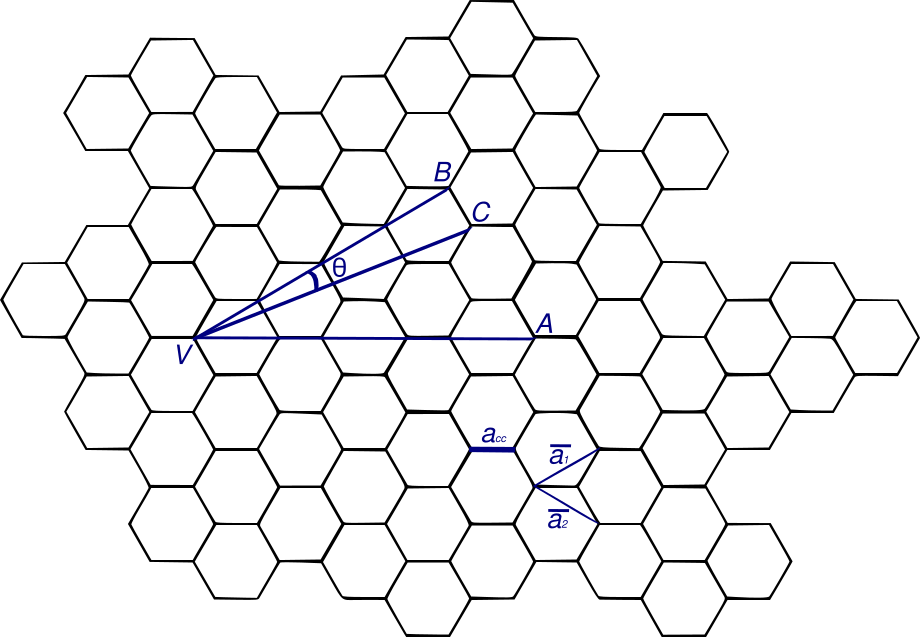
\includegraphics[width=0.7\textwidth]{images/panal1.png}
    \caption{Caption}
    \label{fig:enter-label}
\end{figure}
\begin{align}
    \vec{C_v} = n\vec{a_1} + m \vec{a_2} = (n, m) , \ \textit{tal que} \ |\vec{a_1}| = |\vec{a_1}| = \sqrt{3} a_{cc} \\
     |\vec{C_v}| = a_{cc}\sqrt{n^2 + m^2 + mn} 
\end{align}

en coordenadas cartesianas
\begin{align}
    \vec{C_v} = \frac{a_{cc}\sqrt{3}}{2}(\sqrt{3} \hat{i} +  \hat{j})
\end{align}
El diámetro del nanotubo seria $d=|C_v|/\pi$, ademas se deduce de las graficas y ecuaciones
\begin{align}
    \cos{\theta} = \frac{2n+m}{2\sqrt{n^2 + m^2 + mn}}
\end{align}


\begin{itemize}
\item Explicación detallada de los métodos de simulación por dinámica molecular empleados en el estudio.
\item Descripción del potencial empírico utilizado y su validación mediante comparación con valores experimentales.
\item Consideraciones adicionales en los cálculos de energía y estructura de moléculas de hidrocarburos y superficies de diamante.
\end{itemize}

\section{Resultados y discusión}
\begin{itemize}
\item Presentación y análisis de los resultados obtenidos a partir de la simulación por dinámica molecular.
\item Discusión de las energías de adsorción de moléculas en superficies de diamante y su relevancia para el crecimiento de SWNT.
\item Análisis de las propiedades de energía y estructura de los SWNT simulados, comparándolos con los valores experimentales cuando estén disponibles.
\item Interpretación de los resultados y su relación con los mecanismos de crecimiento y síntesis de SWNT.
\end{itemize}

\section{Conclusiones}
\begin{itemize}
\item Resumen de los hallazgos más relevantes del estudio.
\item Reflexión sobre la contribución del enfoque de simulación por dinámica molecular en el entendimiento del crecimiento y síntesis de SWNT.
\item Posibles direcciones futuras de investigación y mejoras en los métodos de simulación.
\end{itemize}

\printbibliography

\end{document} 
